\documentclass[10pt,aspectratio=43]{ISAE-Beamer}
\usefonttheme[onlymath]{serif}
\usepackage{media9}
% === PACKAGES === %

\usepackage{
amsmath,
amssymb,
amsthm,
dsfont,
fontawesome,
multimedia,
tcolorbox,
ulem
}

%\usepackage{tikz}
\usetikzlibrary{arrows}
\usetikzlibrary{decorations.pathmorphing}
\usepackage{hyperref}

% ANDREA
%\usepackage{arydshln,mathtools}
%\usepackage{bm} %=>Fatal error occurred, no output PDF file produced!
% \usepackage[backend=bibtex,doi=false,isbn=false,url=false,eprint=false]{biblatex}
% Package biblatex Error: Incompatible package 'ucs'
% \bibliography{../mybibliography} %

%\bibliography{WavesPHSAnaNumNEW}

% === COLORS === %

\newcommand{\blue}[1]{\textcolor{blue}{#1}}
\colorlet{darkpurple}{purple!80!black}
\newcommand{\darkpurple}[1]{\textcolor{darkpurple}{#1}}
\colorlet{darkgreen}{green!50!black}
\newcommand{\green}[1]{\textcolor{darkgreen}{#1}}
\colorlet{darkorange}{orange!90!black}
\newcommand{\orange}[1]{\textcolor{darkorange}{#1}}
\newcommand{\purple}[1]{\textcolor{purple}{#1}}
\newcommand{\red}[1]{\textcolor{red}{#1}}

% === MACROS === %

% = A = %
\newcommand{\Alpha}{\vector{\alph}}
\newcommand{\alphap}{\alph_p}
\newcommand{\Alphaq}{\Alpha_q}
\newcommand{\Alphav}{\boldsymbol{\alpha}_v}
\newcommand{\alp}{\vector{\alph}}
\renewcommand{\alph}{\purple{\alpha}}



% = B = %
\newcommand{\biblio}{\blue{\tiny\faBook}}

\newcommand{\bm}{\boldsymbol} 
% = C = %
\renewcommand{\check}{\red{\checkmark}}
\newcommand{\curl}{\vector{\rm curl}}

% = D = %
\newcommand{\D}{\green{\mc D}}
\newcommand{\dd}{{\rm ~d}}
\renewcommand{\div}{{\rm div}}
\newcommand{\divs}{{\mbox{\rm \tiny div}}}
\newcommand{\dsp}{\displaystyle}
\DeclareMathOperator*{\Div}{Div}
% = E = %
\newcommand{\E}{\purple{\mc E}}
\newcommand{\Eo}{\orange{E}}
\newcommand{\e}{\vector{\eff}}
\newcommand{\eff}{\purple{e}}
\newcommand{\eg}{\textit{e.g.~}}
\renewcommand{\emph}{\textbf}
\newcommand{\epso}{\orange{\epsilon}}
\newcommand{\eqdef}{:=}

\newcommand{\energy}[1]{\frac{1}{2} \int_{\Omega} \left\{ #1 \right\} \dd\Omega}

% = F = %
\newcommand{\F}{\darkpurple{\mc F}}
\newcommand{\f}{\darkpurple{\vector{f}}}
\newcommand{\flo}{\darkpurple{f}}
\newcommand{\Forall}{ \quad \forall }

% = G = %
\newcommand{\grad}{\vector{\rm grad}}
\newcommand{\graph}{\mbox{\rm Graph}}
\DeclareMathOperator*{\Grad}{Grad}

% = H = %
\renewcommand{\H}{\mathbf{H}}
\newcommand{\Ham}{\green{\mc H}}
\DeclareMathOperator*{\Hess}{Hess}

% = I = %
\newcommand{\idea}{\raisebox{-0.1cm}{\textcolor{yellow!80!red}{\LARGE\faLightbulbO}}~}
\newcommand{\ie}{\textit{i.e.~}}
\newcommand{\inner}[3][]{\ensuremath{\left\langle #2, \, #3 \right\rangle_{#1}}}


% = J = %
\newcommand{\J}{\green{\mc J}}

% = K = %

% = L = %
\renewcommand{\L}{\mathbf{L}}
\newcommand{\LambdaTens}{\orange{\overline{\overline{\boldsymbol \lambda}}}}

% = M = %
\newcommand{\matl}{\left(\begin{matrix}}
\newcommand{\matr}{\end{matrix}\right)}
\newcommand{\mc}{\mathcal }

% = N = %
\newcommand{\n}{\vector{n}}
\newcommand{\nuo}{\blue{{\boldsymbol \nu}}}
\newcommand{\nol}{\left\Vert}
\newcommand{\nor}{\right\Vert}
\newcommand*{\norm}[1]{\ensuremath{\left\|#1\right\|}}

% = O = %
\newcommand{\one}{\mathds{1}}

% = P = %
\renewcommand{\P}{\mathbb{P}}
\newcommand{\pbl}{\left[}
\newcommand{\pbr}{\right]}
\newcommand{\psl}{\left\langle}
\newcommand{\psr}{\right\rangle}

% = Q = %

% = R = %
\newcommand{\R}{\mathbb{R}}
\newcommand{\rhoo}{\orange{\rho}}

% = S = %
\newcommand{\s}{\vector{s}}
\renewcommand{\S}{\green{\mc S}}

% = T = %
\newcommand{\Tens}{\orange{\overline{\overline{\boldsymbol T}}}}

% = U = %
\renewcommand{\u}{\blue{{\boldsymbol u}}}
\newcommand{\uv}{\blue{\vector{u}}}
\renewcommand{\U}{\green{\mc U}}

% = V = %
\renewcommand{\v}{\vector{v}}
\renewcommand{\vector}[1]{\overrightarrow{\mathbf{\boldsymbol #1}}}

% = W = %
\newcommand{\warning}{\red{\faWarning}~}

% = X = %
\newcommand{\x}{\vector{x}}

% = Y = %
\newcommand{\y}{\red{{\boldsymbol y}}}
\newcommand{\yv}{\red{\vector{y}}}

% = Z = %
\newcommand{\Zo}{\orange{Z}}

% == images == %

\graphicspath{{./imagesPFEM/}}

% === TITLE INFORMATIONS === %


\title[PFEM 4 PHS]{\blue{Numerics for PH-PDEs}\\
  \small{The Partitioned Finite Element Method, a structure-preserving method for physics-based PDEs with boundary control.}}

\institute[ISAE-SUPAERO]{\inst{1} ISAE-SUPAERO, Universit\'e de Toulouse \and \inst{2} Instituto Tecnológico de Aeronáutica \and \inst{3} Institut Polytechnique de Grenoble}

\author[D. Matignon]{D. Matignon\inst{1} {\and} F.L. Cardoso-Ribeiro\inst{2} {\and} L. Lefèvre\inst{3}}

\date{19/07/2022}

%\thanks{
\includegraphics[height=0.1\textwidth]{INFIDHEM-logo} \hspace{.5cm}
%
\includegraphics[height=0.1\textwidth]{logoITA.png} \hspace{.5cm}
%
\includegraphics[height=0.1\textwidth]{logoLCIS.png}
%}

\begin{document}

\maketitle

\begin{frame}{Outline}

\tableofcontents

\end{frame}

\section{Introduction}


\begin{frame}
	\frametitle{Main Objective}
	\onslide<1->\begin{block}{Aim:}
		\textit{\green{Simulate}} \textit{\blue{complex open physical systems}} by ensuring the \textit{\red{conservation of the \emph{\underline{power balance}}}} for a chosen functional: the \emph{Hamiltonian}.
	\end{block}\vfill
	
	\begin{itemize}
		\item<2->
		\green{\underline{\textit{Finite Element Method:}}}
		
		$\rightarrow$ \emph{Complex geometries} are allowed.
		
		$\rightarrow$ A wide range of \emph{implementation} tools are available.\vfill
		
		\item<3->
		\blue{\underline{\textit{Port-Hamiltonian Systems (PHS):}}}
		
		$\rightarrow$ Model \emph{``energy'' exchanges} between simpler open subsystems.
		
		$\rightarrow$ The power balance is \textit{encoded} in a \emph{Stokes-Dirac structure}.\vfill
		
		\item<4->
		\red{\underline{\textit{Partitioned Finite Element Method (PFEM):}}}
		
		$\rightarrow$ It approximates the Stokes-Dirac structure into a \emph{Dirac structure}.
		
		$\rightarrow$ The \emph{discrete Hamiltonian} satisfies a ``discrete'' power balance.
	\end{itemize}
	\vfill
	\onslide<4->{\small
		\blue{A Partitioned Finite-Element Method for power-preserving discretization of open systems of conservation laws}
		
		\textbf{\quad Cardoso-Ribeiro F.L., Matignon D., Lef\`evre L.}
		
		\quad  \textit{IMA J. Mathematics of Control and Information, vol.38(2) , pp. 493--533 (2021)}
	}
\end{frame}


\begin{frame}{Change of paradigm?}
	
	\begin{center}
	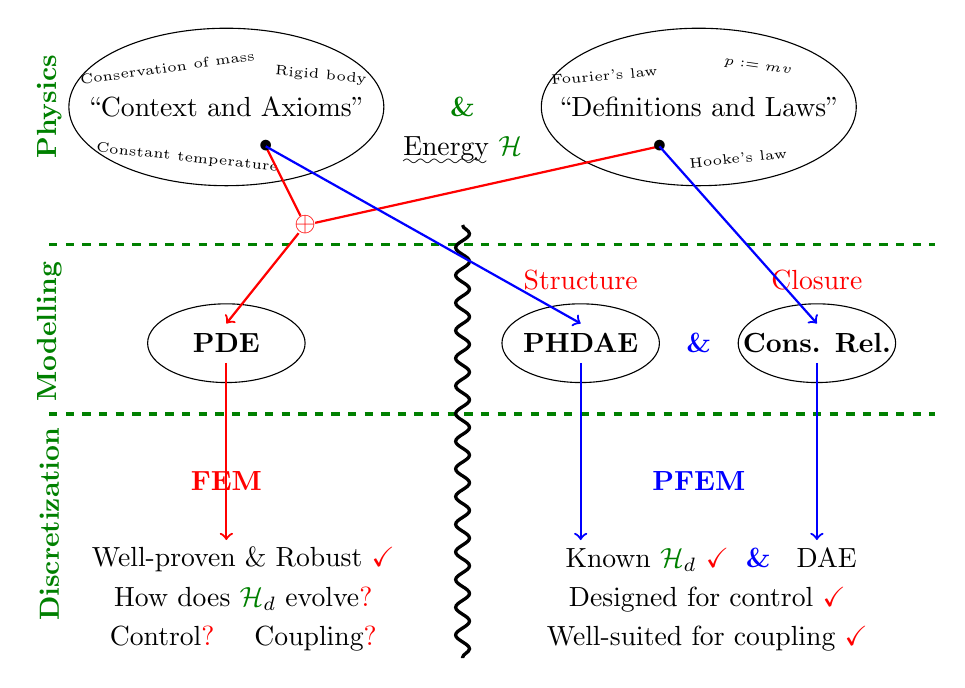
\begin{tikzpicture}[scale=1]
		\onslide<1->
		\draw (-3,0) node{``Context and Axioms''} ellipse (2cm and 1cm); 
		\node[rotate=8] at (-3.75,0.5) {\tiny Conservation of mass};
		\node[rotate=-5] at (-1.8,0.4) {\tiny Rigid body};
		\node[rotate=-6] at (-3.5,-0.65) {\tiny Constant temperature};
		\draw (0,0) node{\green{${\boldsymbol \&}$}};
		\draw (0,-0.25)  node[below]{\uwave{Energy} $\Ham$}; 
		\draw (3,0) node{``Definitions and Laws''} ellipse (2cm and 1cm); 
		\node[rotate=-8] at (3.75,0.5) {\tiny $p \eqdef mv$};
		\node[rotate=5] at (1.8,0.4) {\tiny Fourier's law};
		\node[rotate=6] at (3.5,-0.65) {\tiny Hooke's law};
		\draw[darkgreen,very thick,dashed] (-5.25,-1.75) -- (6,-1.75);
		\draw[darkgreen,very thick,dashed] (-5.25,-3.9) -- (6,-3.9);
		\draw[decorate,decoration=snake,very thick] (0,-1.5) -- (0,-7); 
		\draw[darkgreen] (-5.25,0) node{\rotatebox{90}{\textbf{Physics}}};
		\draw[darkgreen] (-5.25,-2.85) node{\rotatebox{90}{\textbf{Modelling}}};
		\draw[darkgreen] (-5.25,-5.3) node{\rotatebox{90}{\textbf{Discretization}}};
		
		\onslide<2->
		\draw (-3,-3) node{\emph{PDE}} ellipse (1cm and 0.5cm); 
		\draw[red,thick] (-2.5,-0.5) -- (-2,-1.5); 
		\draw[->,red,thick] (-2,-1.5) -- (-3,-2.75); 
		\draw[red,thick] (2.5,-0.5) -- (-2,-1.5); 
		\draw[white,fill=white] (-2,-1.5) node{$\red{\oplus}$} circle (0.125cm); 
		\draw[->,red,thick] (-3,-3.25) -- (-3,-5.5); 
		\draw[red] (-3,-4.75) node{\textbf{FEM}}; 
		\draw (-3,-5.75) node{\; \; Well-proven \& Robust \check}; 
		\draw (-3,-6.25) node{\; \; How does $\Ham_d$ evolve\red{?}}; 
		\draw (-3,-6.75) node{\; \; Control\red{?} \quad Coupling\red{?}}; 
		\draw (-2.5,-0.5) node{$\bullet$}; 
		\draw (2.5,-0.5) node{$\bullet$}; 
		
		\onslide<3->
		\node at (1.5,-2.2) {\red{Structure}};
		\draw (1.5,-3) node{\emph{PHDAE}} ellipse (1cm and 0.5cm); 
		\draw[blue] (3,-3) node{${\boldsymbol \&}$}; 
		\node at (4.5,-2.2) {\red{Closure}};
		\draw (4.5,-3) node{\emph{Cons. Rel.}} ellipse (1cm and 0.5cm); 
		\draw[->,blue,thick] (-2.5,-0.5) -- (1.5,-2.75); 
		\draw[->,blue,thick] (2.5,-0.5) -- (4.5,-2.75); 
		\draw[->,blue,thick] (1.5,-3.25) -- (1.5,-5.5); 
		\draw[->,blue,thick] (4.5,-3.25) -- (4.5,-5.5); 
		\draw[blue] (3,-4.75) node{\textbf{PFEM}}; 
		\draw (3,-5.75) node{\; \; Known $\Ham_d$ \check \; $\blue{\boldsymbol \&}$ \; DAE \warning}; 
		\draw (3,-6.25) node{\; Designed for control \check}; 
		\draw (3,-6.75) node{\; Well-suited for coupling \check}; 
		
		\onslide<1->
	\end{tikzpicture}
	\end{center}
\end{frame}

\begin{frame}{Port-Hamiltonian Systems (PHS)}
	
	\begin{itemize}
		\item<1->
		The \emph{energy variables} $\alp$ (vector field);
		\item<1->
		The \emph{Hamiltonian} $\Ham(\alp(t))$ (positive functional);
		\item<2->
		The \emph{co-energy variables} $\e_{\alp} \eqdef \delta_{\alp} \Ham$ (vector field), \\ \qquad $\leadsto$ the variational derivative of $\Ham$ w.r.t $\alp$;
		\item<3->
		The \emph{\textit{structure} operator} $J$ (linear and \textit{formally skew-symmetric});
		\item<3->
		The \emph{resistive/dissipative operator} $R$ (linear and \textit{positive});
		\item<4->
		The \emph{control operator} $B$ (linear);
		\item<4->
		The \emph{input} $\u$ and the \emph{collocated output} $\y$ (boundary fields);
		\item<5->
		The \emph{dynamical system}:
		\begin{tcolorbox}
			\centering
			$
			\left\{\begin{array}{l}
				\partial_t \alp(t) = \left( J - R \right) \e_{\alp}(t) + B \u(t), \\
				\y(t) = B^* \e_{\alp}(t).
			\end{array}\right.
			$
		\end{tcolorbox}
	\end{itemize}
	\onslide<6->
	\begin{alertblock}{\textbf{Lossy Power Balance}}
		\centering
		$
		\frac{\rm d}{{\rm d}t} \Ham(\alp(t)) = - \psl R \e_{\alp}(t), \e_{\alp}(t) \psr_J + \psl \u(t), \y(t) \psr_B \; \le \; \psl \u(t), \y(t) \psr_B.
		$
	\end{alertblock}
	\hspace{-6pt}\warning\hspace{-6pt} Although \textbf{\red{the underlying geometry}} is well-determined with the above equality, \emph{constitutive relations} between $\alp$ and $\e_{\alp}$ are also needed to solve the system!
	
\end{frame}


\section{Linear Wave equations: towards PH-DAEs and PH-ODEs}

%%%%%%%%%%%%%%%%%%%% SS Discretieaion PH DAEs
\subsection{Discretization in terms of energy and co-energy variables: PH-DAEs}

\begin{frame}{Conservative System: Wave as PH-DAE}
	
	\onslide<1-> \textbf{\red{Deflection} $w$ of a 2D-membrane, \blue{\textit{boundary deflection velocity} as control}.}\vfill
	\onslide<2-> Its total energy is given by the sum of the potential \& kinetic energies:\vfill
	\centering
	$
	\dsp \Ham(\alp_q, \alph_p) 
	\eqdef \frac{1}{2} \int_\Omega \left( \alp_q \cdot \Tens \cdot \alp_q + \frac{1}{\rhoo} \alph_p^2 \right).
	$
	\begin{itemize}
		\item<3->
		$\rhoo$ the \textit{mass density} of the medium and $\Tens$ the \textit{Young modulus} tensor;
		\item<3->
		$\alph_p \eqdef \rhoo\,\partial_t w$ the \textit{linear momentum} and $\alp_q \eqdef \grad \left( w \right)$ the \textit{strain};
		\item<4->
		$\e_q \eqdef \delta_{\alp_q} \Ham = \Tens \cdot \alp_q$ the \textit{stress};
		\item<4->
		$\eff_p \eqdef \delta_{\alph_p} \Ham = \frac{\alph_p}{\rhoo} = \partial_t w$ the \blue{\it deflection velocity} and $\u \eqdef \eff_p$;
		\item<5->
		$\y \eqdef \e_q \cdot \n$ the output \red{\it normal stress}.
	\end{itemize}
	\onslide<6->
	{\small
		$$
		\left\{\begin{array}{rl}
			\rhoo \partial_{tt}^2 w &= \div \left( \Tens \cdot \grad \left( w \right) \right), \\
			\u &= \partial_t w, \\
			\y &= \left( \Tens \cdot \grad \left( w \right) \right) \cdot \n.
		\end{array}\right.
		\onslide<7->
		\hspace{-10pt}
		\Leftrightarrow
		\hspace{-2pt}
		\left\{\begin{array}{rl}
			\partial_t \alp_q &= \grad \left( \eff_p \right), \\
			\partial_t \alph_p &= \div \left( \e_q \right),
		\end{array}\right.
		\hfill
		\&
		\hfill
		\left\{\begin{array}{rl}
			\u &= \eff_p, \\
			\y &= \e_q \cdot \n.
		\end{array}\right.
		$$}
	\onslide<8->
	\begin{alertblock}{Lossless \textbf{Power Balance}}
		\centering
		$
		\frac{\rm d}{{\rm d}t}\Ham (\alp_q, \alph_p) 
		= \psl \y, \u \psr_{H^{-\frac{1}{2}},H^{\frac{1}{2}}}.
		$
	\end{alertblock}
	
\end{frame}

\begin{frame}{Conservative System: PFEM strategy}
	
	\onslide<1->
	\begin{block}{The strategy follows:}
		\begin{enumerate}
			\item<2->
			Write the \textbf{weak formulation};
			\item<3->
			Apply an accurate \textbf{Stokes (Green) identity} (such that $\u$ ``appears'');
			\item<4->
			Project on a finite-dimensional space thanks to \textbf{FEM}.
		\end{enumerate}
	\end{block}
	\vfill
	\onslide<5-> For all test functions $\v_q$, $v_p$ and $v_\partial$ (smooth enough):
	$$
	~\hspace{-0.5cm}\left\{\begin{array}{l}
		\dsp \psl \partial_t \alp_q, \v_q \psr_{\L^2} = \psl \grad \left( \eff_p \right), \v_q \psr_{\L^2}, \\
		\dsp \psl \partial_t \alph_p, v_p \psr_{L^2} = \psl \div \left( \e_q \right), v_p \psr_{L^2}, \\
		\dsp \psl \y, v_\partial \psr_{H^{-\frac{1}{2}},H^{\frac{1}{2}}} = \psl \e_q \cdot \n, v_\partial \psr_{H^{-\frac{1}{2}},H^{\frac{1}{2}}}.
	\end{array}\right.
	$$
	\onslide<6-> Applying Green's formula on the 1st line and using the definition of $\u$:
	$$
	\psl \partial_t \alp_q, \v_q \psr_{\L^2} = - \psl \eff_p, \div \left( \v_q \right) \psr_{L^2} 
	+ \psl \v_q \cdot \n, \u \psr_{H^{-\frac{1}{2}},H^{\frac{1}{2}}}.
	$$
	\vfill
	\onslide<7-> 
	\begin{tcolorbox}
		Green's formula applied on the 2nd line would lead to normal stress control $\u = \e_q \cdot \n$. The energy variables are \textbf{partitioned} accordingly.
	\end{tcolorbox}
	
\end{frame}

\begin{frame}{Conservative System: FEM Application}
	
	The energy, co-energy, boundary and test functions of the \textit{same} index are discretized by using the \textit{same} bases, either scalar- or \textbf{vector}-valued:
	$$
	\begin{array}{ll}
		\onslide<1-> \alp_q^{ap}(t,\x) \eqdef \sum_{\ell=1}^{N_q} \vector{\phi}_q^\ell(\x) \alph_q^\ell(t) = \vector{\Phi}_q^\top \cdot \underline{\alph}_q(t), &
		\onslide<2-> \e_q^{ap}(t,\x) =  \vector{\Phi}_q^\top \cdot \underline{\eff}_q(t), \\
		\onslide<3->\alph_p^{ap}(t,\x) \eqdef \sum_{k=1}^{N_p} \varphi_p^k(\x) \alph_p^k(t) = {\boldsymbol \phi}_p^\top \cdot \underline{\alph}_p(t), &
		\eff_p^{ap}(t,\x) = {\boldsymbol \phi}_p^\top \cdot \underline{\eff}_p(t), \\
		\onslide<4->\u^{ap}(t,\s) \eqdef \sum_{m=1}^{N_{\partial}} \psi^m(\s) \u^m(t) = {\boldsymbol \Psi}^\top \cdot \underline{\u}(t), & 
		\y^{ap}(t,\s) = {\boldsymbol \Psi}^\top \cdot \underline{\y}(t),
	\end{array}
	$$
	\onslide<1-> with $\vector{\Phi}_q$ an $N_q \times 2$ matrix, \onslide<3-> ${\boldsymbol \phi}_p$ an $N_p \times 1$ matrix \onslide<4-> and ${\boldsymbol \Psi}$ an $N_{\partial} \times 1$ matrix.\vfill
	\onslide<5->
	\begin{block}{The discretized system (giving the structure) then reads:}
		\centering
		$
		\left\{\begin{array}{l}
			\vector{M}_q \cdot \frac{\rm d}{{\rm d}t}\underline{\alph}_q(t) = D \cdot \underline{\eff}_p(t) + B \cdot \underline{\u}(t), \\
			M_p \cdot \frac{\rm d}{{\rm d}t}\underline{\alph}_p(t) = -D^\top \cdot \underline{\eff}_q(t), \\
			M_\partial \cdot \underline{\y}(t) = B^\top \cdot \underline{\eff}_q(t),
		\end{array}\right.
		$
	\end{block}
	\flushleft\onslide<6-> where:
	$$
	\begin{array}{c}
		\vector{M}_q \eqdef \int_\Omega \vector{\Phi}_q \cdot \vector{\Phi}_q^\top, \qquad
		M_p \eqdef \int_\Omega {\boldsymbol \phi}_p \cdot {\boldsymbol \phi}_p^\top, \qquad
		M_\partial \eqdef \int_{\partial\Omega} {\boldsymbol \Psi} \cdot {\boldsymbol \Psi}^\top, \\
		~ \\
		D \eqdef - \int_\Omega \div\left( \vector{\Phi}_q \right) \cdot {\boldsymbol \phi}_p^\top, \qquad
		B \eqdef \int_{\partial\Omega} \left( \vector{\Phi}_q \cdot \n \right) \cdot {\boldsymbol \Psi}^\top.
	\end{array}
	$$
\end{frame}


\begin{frame}{Conservative System: Power Balance}
	
	\onslide<1->
	\begin{alertblock}{Finite-Dimensional extended structure operator}
		\centering
		$
		\green{\J}_d \eqdef \matl 0 & D & B \\ -D^\top & 0 & 0 \\ -B^\top & 0 & 0 \matr.% \quad \Longrightarrow \quad \D_d \eqdef \graph \left( \green{\J}_d \right).
		$
	\end{alertblock}
	\onslide<2-> \warning The inner product on $\R^{N_q}$, $\R^{N_p}$ and $\R^{N_\partial}$ has to be taken w.r.t. the mass matrices $\vector{M}_q$, $M_p$ and $M_\partial$: \eg $\psl \v_1, \v_2 \psr_{N_q} \eqdef \v_2^\top \cdot \vector{M}_q \cdot \v_1$.\vspace{-2pt}
	\onslide<3-> 
	\begin{alertblock}{Discrete Hamiltonian}
		\centering
		$
		\green{\Ham}_d \left( \underline{\alph}_q, \underline{\alph}_p \right) \eqdef \Ham \left( \alp_q^{ap}, \alph_p^{ap} \right) = \frac{1}{2} \left( \underline{\alph}_q^\top \cdot \vector{M}_{\Tens} \cdot \underline{\alph}_q + \underline{\alph}_p^\top \cdot M_{\frac{1}{\rhoo}} \cdot \underline{\alph}_p \right),
		$\vfill
		\onslide<4-> $\vector{M}_{\Tens} \eqdef \int_\Omega \vector{\Phi}_q \cdot \Tens \cdot \vector{\Phi}_q^\top$ \qquad \& \qquad $M_{\frac{1}{\rhoo}} \eqdef \int_\Omega \frac{1}{\rhoo} {\boldsymbol \phi}_p \cdot {\boldsymbol \phi}_p^\top$.
	\end{alertblock}
	\onslide<5-> \textbf{Constitutive relations}: \quad $\vector{M}_q \cdot \underline{\eff}_q = \vector{M}_{\Tens} \cdot \underline{\alph}_q$ \quad \& \quad $M_p \cdot \underline{\eff}_p = M_{\frac{1}{\rhoo}} \cdot \underline{\alph}_p$ \hfill \check \check \vfill
	\onslide<6-> Denote $\underline{\flo} \eqdef \matl \frac{\rm d}{{\rm d}t}\underline{\alph}_q, & \frac{\rm d}{{\rm d}t}\underline{\alph}_p, & -\underline{\y} \matr^\top$ and $\underline{\eff} \eqdef \matl \underline{\eff}_q, & \underline{\eff}_p, & \underline{\u} \matr^\top$, then:
	\begin{alertblock}{Discrete Lossless \textbf{Power Balance}}
		\centering
		$
		%\matl \underline{\flo} \\ \underline{\eff} \matr \in \D_d \; \Rightarrow \; \psl \underline{\flo}, \underline{\eff} \psr_{N_p, N_q, N_\partial} = 0 
		%\; \Rightarrow \; 
		\frac{\rm d}{{\rm d}t}\Ham_d \left( \underline{\alph}_q, \underline{\alph}_p \right) = \underline{\u}^\top \cdot M_\partial \cdot \underline{\y}.
		$
	\end{alertblock}
	
\end{frame}


\begin{frame}{A Proof of the Discrete Power Balance}
	Since by definition the discrete Hamiltonian reads:
	$$\green{\Ham}_d \left( \underline{\alph}_q, \underline{\alph}_p \right)  = \frac{1}{2} \left( \underline{\alph}_q^\top \cdot \vector{M}_{\Tens} \cdot \underline{\alph}_q + \underline{\alph}_p^\top \cdot M_{\frac{1}{\rhoo}} \cdot \underline{\alph}_p \right),$$
	we can compute its time derivative along the trajectories:
	\begin{eqnarray*}
		\frac{\rm d}{{\rm d}t}\Ham_d \left( \underline{\alph}_q, \underline{\alph}_p \right)
		&=& ({\frac{\rm d}{{\rm d}t}\underline{\alph}_q})^\top \cdot \vector{M}_{\Tens} \cdot \underline{\alph}_q + ({\frac{\rm d}{{\rm d}t}\underline{\alph}_p})^\top \cdot M_{\frac{1}{\rhoo}} \cdot \underline{\alph}_p ,\\
		&=& ({\frac{\rm d}{{\rm d}t}\underline{\alph}_q})^\top \cdot \vector{M}_q \cdot \underline{\eff}_q + ({\frac{\rm d}{{\rm d}t}\underline{\alph}_p})^\top \cdot M_p \cdot \underline{\eff}_p ,\\
		&=& (\vector{M}_q\cdot {\frac{\rm d}{{\rm d}t}\underline{\alph}_q})^\top \cdot  \underline{\eff}_q + (M_p \cdot {\frac{\rm d}{{\rm d}t}\underline{\alph}_p})^\top \cdot \underline{\eff}_p ,\\
		&=& (  D \cdot \underline{\eff}_p(t) + B \cdot \underline{\u}(t) )^\top \cdot  \underline{\eff}_q + ( -D^\top \cdot \underline{\eff}_q(t)  )^\top \cdot \underline{\eff}_p ,\\
		&=&  \underline{\u}(t)^\top \cdot  B^\top\cdot  \underline{\eff}_q\\
		&=& \underline{\u}(t)^\top \cdot M_\partial \cdot\underline{\y}(t) . \qed
	\end{eqnarray*}
\end{frame}

\begin{frame}{PFEM for pHs gives rise to PH-DAEs}
	
	Summarizing the main steps: discretization of the structure and of the constitutive relations are made separately.
	
	\begin{block}{The discretized system is a PH-DAE:}
		\centering
		$
		\left\{\begin{array}{l}
			\vector{M}_q \cdot \frac{\rm d}{{\rm d}t}\underline{\alph}_q(t) = D \cdot \underline{\eff}_p(t) + B \cdot \underline{\u}(t), \\
			M_p \cdot \frac{\rm d}{{\rm d}t}\underline{\alph}_p(t) = -D^\top \cdot \underline{\eff}_q(t), \\
			M_\partial \cdot \underline{\y}(t) = B^\top \cdot \underline{\eff}_q(t),
		\end{array}\right.
		$
		
		together with
		
		$
		\left\{\begin{array}{l}
			\vector{M}_q \cdot \underline{\eff}_q(t) = \vector{M}_{\Tens} \cdot \underline{\alph}_q(t), \\
			M_p \cdot \underline{\eff}_p(t) = M_{\frac{1}{\rhoo}} \cdot \underline{\alph}_p(t)
		\end{array}\right.
		$
	\end{block}
	
	
\end{frame}


\subsection{Convergence of PFEM}

\begin{frame}{Convergence rate: theory}
	
	\onslide<1->
	\begin{block}{Theorem (Haine, Matignon \& Serhani,  2020)}
		
		Let $\kappa\ge\delta$ be an integer, where $\delta=0$ if $\Omega$ is convex and $1$ otherwise, and $T>0$.
		
		Let $\matl {\Alphaq}_0 \\ {\alphap}_0 \matr \in \mathcal Z_\kappa := \matl \Tens & 0 \\ 0 & \frac{1}{\rhoo} \matr^{-1} \left[ \begin{matrix} \H_\divs^{\kappa+1}(\Omega) \\ H^{\kappa+1}(\Omega) \end{matrix} \right]$, $\u \in C^2([0,\infty);H^{\kappa+1}(\partial\Omega))$.
		
		Let $\matl \Alphaq^{ap}(0) \\ \alphap^{ap}(0) \matr$, $\u^{ap}$ be their interpolations with $\left(\mathbb P^{k}\right)^N \times \mathbb P^{\ell} \times \mathbb P^{m}$.
		
		Let ${\bf E}(t) \eqdef \nol \matl (\Alphaq-\Alphaq^{ap})(t), & (\alphap-\alphap^{ap})(t) \matr^\top \nor_{\L^2 \times L^2}$,
		
		$\exists C_T>0$, independent of $\matl {\Alphaq}_0 \\ {\alphap}_0 \matr$, and $\u$: for all $h$ and all $t \in [0,T]$
		$$
		{\bf E}(t)
		\le C_T
		h^{\min \left\{ \ell - \delta \, ; \, k \, ; \, m \right\}} 
		\left( \nol \matl \Alphaq \\ \alphap \matr \nor_{L^\infty([0,T];\mathcal Z_{\kappa})} 
		+ \nol \u \nor_{L^\infty([0,T];H^{\kappa+1}(\partial\Omega))} \right).
		$$
		The \emph{optimal} order is $\red{\kappa-\delta}$, when $k=\kappa-\delta$, $\ell=\max\{\kappa;1\}$ and $m=\kappa-\delta$.
	\end{block}
	
	\onslide<2->
	$RT_{\kappa-1-\delta} \times \mathbb P^{\kappa} \times \mathbb P^{\kappa-\delta}$ \hfill $BDM_{\kappa-\delta} \times \mathbb P^{\kappa} \times \mathbb P^{\kappa-\delta}$ \hfill $BDFM_{\kappa-\delta} \times \mathbb P^{\kappa} \times \mathbb P^{\kappa-\delta}$~
	
\end{frame}

\begin{frame}{Convergence rate: numerics}
	\begin{figure}
		\centering
		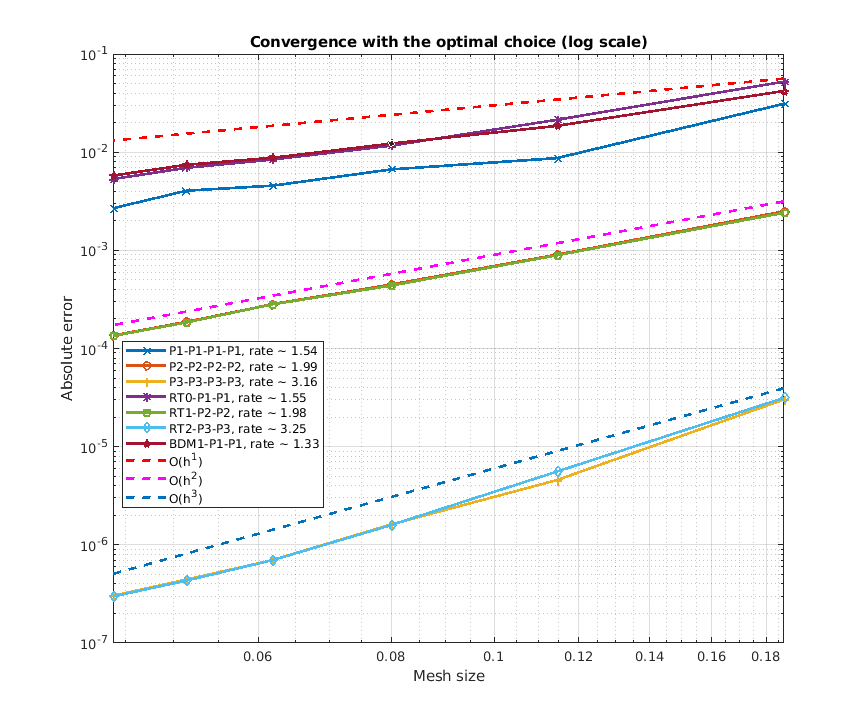
\includegraphics[width=0.9\textwidth]{CVoptimal}
	\end{figure}
	
	
\end{frame}

\begin{frame}{\small A map for choosing the appropriate finite elements: FEEC}
	\begin{figure}
		\centering
		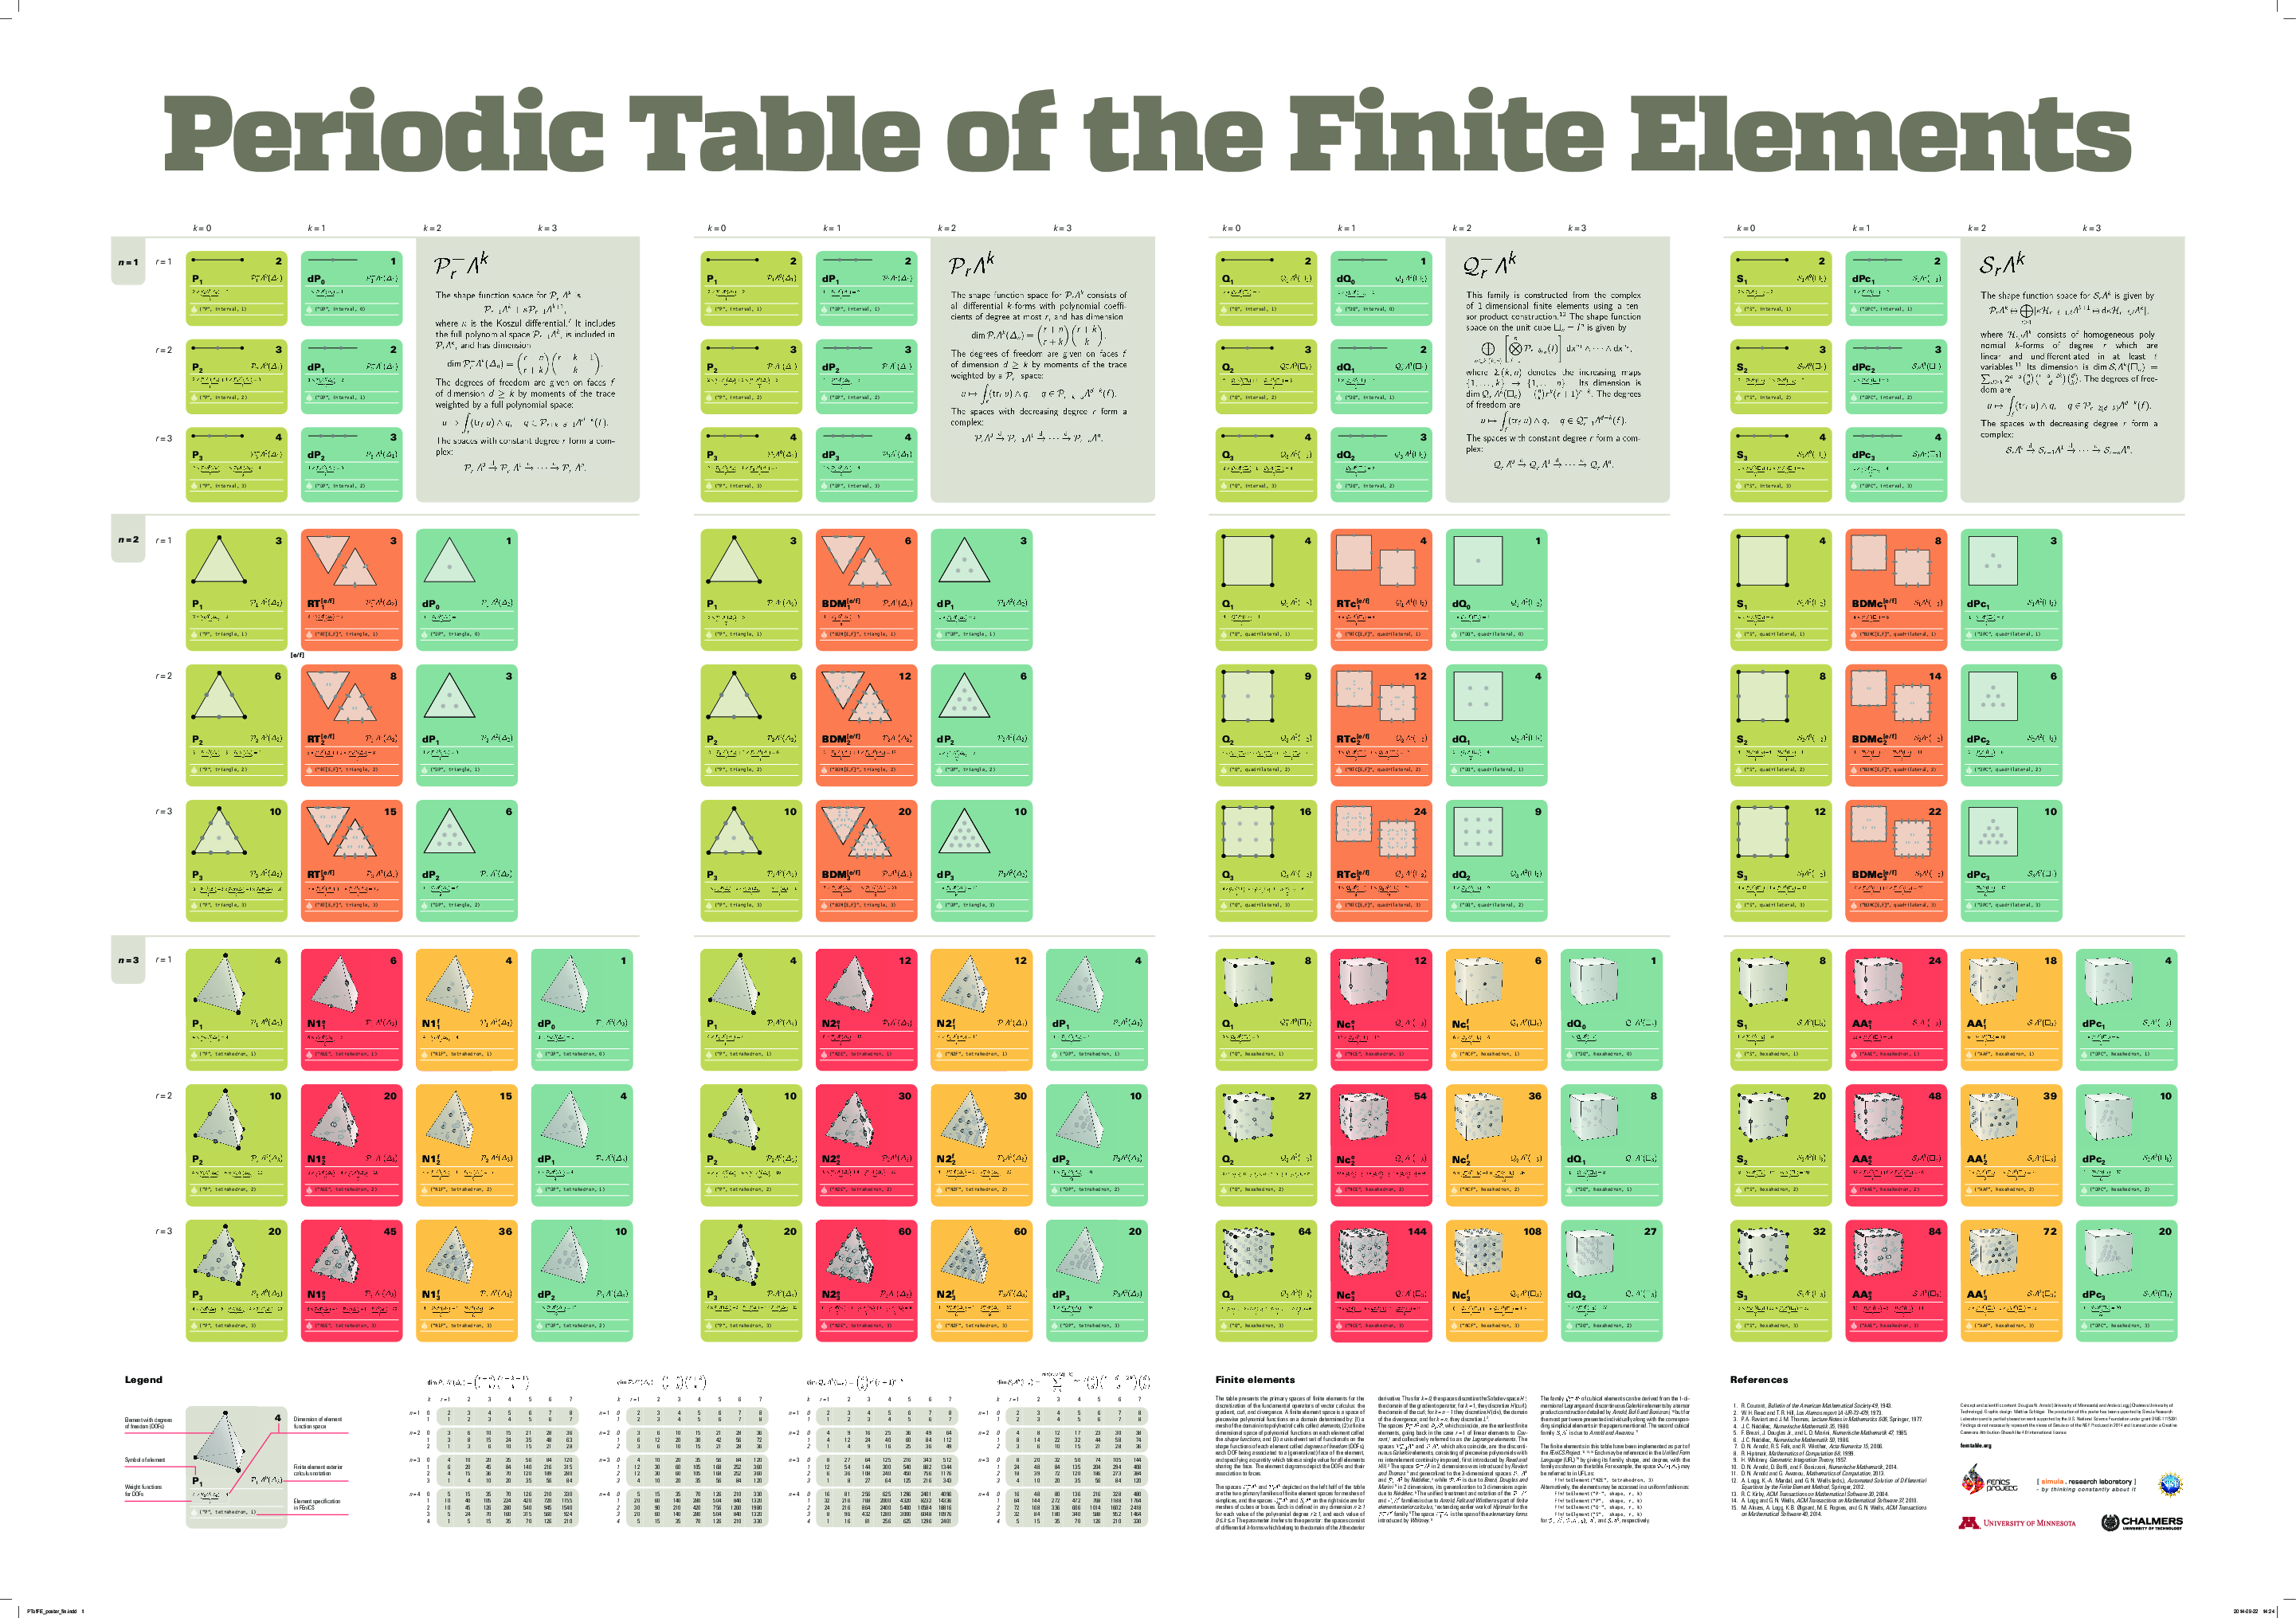
\includegraphics[width=0.9\textwidth]{FenicsFEM}
		
	\end{figure}
\end{frame}

%%%%%%%%%%%%%%%%%%%%%%% SS Boundary Dissipation
\subsection{Application: Boundary Dissipation}


\begin{frame}{Impedance Boundary Condition (IBC)}
	
	\onslide<1-> The Impedance Boundary Condition, with $\Zo\ge0$ on $\partial\Omega$, and $\nuo$ as new control, is considered:\hfill~
	$
	\nuo = \eff_p + \Zo \e_q \cdot \n
	$\hfill~$\Leftrightarrow$\hfill~$\nuo = \partial_t w + \Zo \left( \Tens \cdot \grad \left( w \right) \right) \cdot \n$.~
	\onslide<2-> \warning This kind of dissipation does not \textit{easily} fit in the ``$J-R$ framework''.\vfill
	\onslide<3-> It can be seen as an \textit{output feedback law} $\u = -\Zo \y + \nuo$ in the previous case. 
	\begin{alertblock}{Lossy \textbf{Power Balance}}
		\centering
		$
		\frac{\rm d}{{\rm d}t}\Ham (\alp_q, \alph_p) 
		= - \psl \y, \Zo \y \psr_{H^{-\frac{1}{2}},H^{\frac{1}{2}}} + \psl \y, \nuo \psr_{H^{-\frac{1}{2}},H^{\frac{1}{2}}}.
		$
		\vfill
	\end{alertblock}
	\vfill
	\onslide<4-> Add \textbf{impedance ports} $(\flo_i, \eff_i)$ and \textbf{dissipative constitutive relation} $\eff_i = \Zo \flo_i$,\vfill
	and approximate $\flo_i$ and $\eff_i$ in the boundary FEM basis ${\boldsymbol \Psi}$:
	{\scriptsize~\vspace{-3pt}
		$$
		\matl
		\vector{M}_q & 0 & 0 & 0 & 0 \\
		0 & M_p & 0 & 0 & 0\\
		0 & 0 & M_p & 0 & 0\\
		0 & 0 & 0 & M_\partial & 0\\
		0 & 0 & 0 & 0 & M_\partial 
		\matr
		\matl
		\frac{\rm d}{{\rm d}t}\underline{\alph}_q(t) \\
		\frac{\rm d}{{\rm d}t}\underline{\alph}_p(t) \\
		\underline{\flo}_i(t) \\
		- \underline{\y}(t) 
		\matr
		\hspace{-1.5pt}
		=
		\hspace{-1.5pt}
		\matl
		0 & D & -B & B \\
		-D^\top & 0 & 0 & 0 \\
		B^\top & 0 & 0 & 0 \\
		-B^\top & 0 & 0 & 0 
		\matr
		\matl
		\underline{\eff}_q(t) \\
		\underline{\eff}_p(t) \\
		\underline{\eff}_i(t) \\
		\underline{\nuo}(t) 
		\matr
		$$}\vfill
	and
	\centering
	$
	M_\partial \cdot \underline{\eff}_i = \psl \Zo \psr \cdot \underline{\flo}_i, \qquad \qquad
	$
	with
	$
	\psl \Zo \psr \eqdef \int_{\partial\Omega} \Zo {\boldsymbol \Psi} \cdot {\boldsymbol \Psi}^\top \ge 0.
	$
	\onslide<5-> 
	\begin{alertblock}{Discrete Lossy \textbf{Power Balance}}
		\centering
		$
		\frac{\rm d}{{\rm d}t}\Ham_d \left( \underline{\alph}_q, \underline{\alph}_p \right) =  - \underline{\y}^\top \cdot \psl \Zo \psr \cdot \underline{\y} + \underline{\nuo}^\top \cdot M_\partial \cdot \underline{\y}.
		$
	\end{alertblock}
	
\end{frame}

\begin{frame}{Boundary Dissipation: Simulations}
	
	\begin{minipage}{0.52\textwidth}
		\begin{itemize}
			\item $\rhoo, \; \Tens \not\equiv$ constant;
			\item $\Zo \neq 0$ for $t\ge2$;
			\item Raviart-Thomas FE for $q$-variables;
			\item Lagrange FE for $p$-variables;
			\item Lagrange FE for $\partial$-variables;
		\end{itemize}
	\end{minipage}\hfill
	\begin{minipage}{0.45\textwidth}
		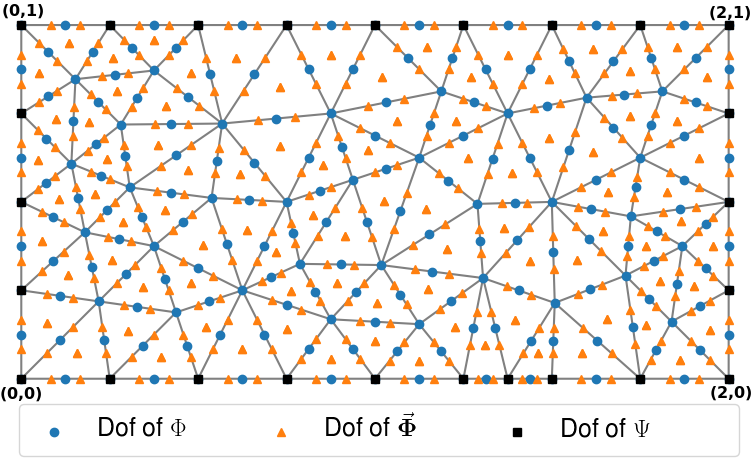
\includegraphics[width=\textwidth, keepaspectratio]{Mesh}
	\end{minipage}
	\vfill
	\begin{center}
		\includemedia[
		width=10cm,height=5cm,
		activate=pageopen,        
		keepaspectratio,          % optionally useful
		transparent,              % optionally useful
		playbutton=plain,
		addresource=/home/andrea/Videos/ENOC2022/simu-wave-boundary.mp4,
		flashvars={
			source=/home/andrea/Videos/ENOC2022/simu-wave-boundary.mp4
			&autoPlay=true
			&loop=true
		}
		]{}{VPlayer.swf}
	\end{center}
	
\end{frame}

\section{Nonlinear wave equation: the 2D Shallow Water Equation}

%%%%%%%%%%%%%%%%%%%%%%% SS SWE as a pHs
\subsection{Modelling: SWE as a pHs}


\begin{frame}{The irrotational shallow water equations}
	\onslide<1->
	* Energy variables:  $\alph_h$ the fluid height, $\alp_v$ the linear momentum,
	
	\onslide<2->
	* \underline{Non-quadratic} and \underline{non-separable}  Hamiltonian functional: 
	\begin{equation*}
		H(\alph_h, \alp_v) = \energy{\frac{1}{\rho} \alph_h \norm{\alp_v}^2 + \rho g \alp_v^2}.
	\end{equation*}
	
	\onslide<3->
	* Dynamical system:
	\begin{equation*} 
		\begin{aligned}
			\frac{\partial}{\partial t}
			\begin{pmatrix}
				\alph_h \\
				\alp_v \\
			\end{pmatrix} &= 
			\begin{bmatrix}
				0 & -\div \\
				-\grad & \bm{0}
			\end{bmatrix}
			\begin{pmatrix}
				\eff_h\\
				\e_v\\
			\end{pmatrix}, \qquad (x,y) \in \Omega = \{x^2 + y^2 \le R \}, \\
			\begin{pmatrix}
				\eff_h\\
				\e_v\\
			\end{pmatrix} &= \begin{pmatrix}
				\delta_{\alp_h} H\\
				\delta_{\alph_v} H\\
			\end{pmatrix} = 
			\begin{pmatrix}
				\frac{1}{2 \rho} \norm{\alph_v}^2 + \rho g \alp_h \\
				\frac{1}{\rho} \alp_h \alph_v
			\end{pmatrix}. 
		\end{aligned}
	\end{equation*}
	
	\onslide<4>{
		* Consider a uniform Neumann boundary control 
		\begin{equation*}
			\u = - \e_v \cdot \n \vert_{\partial\Omega} = - \frac{1}{\rho}\alph_h \alph_v \cdot\n \vert_{\partial\Omega}, \qquad \text{Volumetric inflow rate}.
		\end{equation*}
		The corresponding output reads
		\begin{equation*}
			\y = \eff_h \vert_{\partial\Omega} = (\rho g \alp_h + \frac{1}{2\rho} \norm{\alph_v}^2)\vert_{\partial\Omega}.
		\end{equation*}
	}
	
\end{frame}


\subsection{Numerics: PFEM in the polynomial case}
\begin{frame}
	\onslide<1->
	Polynomial non-linear constitutive relations: off-line computations of the resulting tensors.
	\onslide<2->
	\begin{block}{\textbf{A general result}}
		\centering
		$M_h\cdot \underline{\eff_h}:= \nabla_{\underline{\alph_h}} \Ham_d(\underline{\alph_h}, \underline{\alph_v}) ,$ and 
		$M_v\cdot \underline{\eff_v}:= \nabla_{\underline{\alph_v}} \Ham_d(\underline{\alph_h}, \underline{\alph_v}) .
		$
	\end{block}
	\onslide<3->
	Here quadratic quantities have to be computed in the integrals, namely
	$\underline{q_h}:=\int_\Omega  {\bm{\phi}}_h  \frac{1}{2\,\rho}  \underline{\alph_v}^\top\cdot\vector{\Phi}_v \cdot \vector{\Phi}_v^\top\cdot \underline{\alph_v}$ and
	$
	\underline{q_v}:=\int_\Omega  \vector{\Phi}_v  \frac{1}{\rho}  \underline{\alph_h}^\top\cdot {\boldsymbol \phi}_h \cdot \vector{\Phi}_v^\top\cdot \underline{\alph_v}
	$.
	
	$$
	\Rightarrow 1 \leq i \leq N_h, \quad
	q_h^i(t) = \underline{\alph_v}(t)^\top \cdot \left(\int_\Omega  \phi_h^i \frac{1}{2\,\rho}  \vector{\Phi}_v \cdot \vector{\Phi}_v^\top \right) \cdot \underline{\alph_v}(t) ,
	$$
	$$
	\Rightarrow 1 \leq k \leq N_v, \quad
	q_v^k(t) = \underline{\alph_h}(t)^\top\cdot \left(
	\int_\Omega {\boldsymbol \phi}_h \frac{1}{\rho} {\vector{\phi}_v^k}^\top \cdot \vector{\Phi}_v^\top
	\right) \cdot \underline{\alph_v}(t) .
	$$
	
	{\bf Remark}: the sizes of the vectors and  matrices do match as well (exercise).
	
	$\Longrightarrow$ \red{Off-line computation proves possible!} 
	
	
\end{frame}


\subsection{Application: Boundary Dissipation of a circular water tank}

\begin{frame}{Boundary stabilization of the 2D SWE}
	
	A simple proportional control stabilizes the system around the desired point $\alph_h^{\text{des}}$
	\begin{equation*}
		\u = -k (\y - \y^{\text{des}}), \qquad \y^{\text{des}}= \rho g \alph_h^{\text{des}}, \quad k>0.
	\end{equation*}
	This control law ensures that the Lyapunov functional
	\begin{equation*}
		V = \frac{1}{2} \int_{\Omega}\left\{\frac{1}{2} \rho g (\alph_h - \alph_h^{\text{des}})^2 + \frac{1}{2\rho} \alph_h \norm{\alp_v}^2 \right\} \dd\Omega \ge 0,
	\end{equation*}
	where $\alph_h^{\text{des}}=h^{\text{des}}$, has negative semi-definite time derivative
	\begin{equation*}
		\dot{V} = -k \int_{\partial \Omega}\left(\y - \y^{\text{des}} \right)^2 \dd{\Gamma} \le 0.
	\end{equation*}
\end{frame}

\begin{frame}{Simulation Results for the 2D SWE}
	\begin{equation*}
		\text{Control parameter} \qquad 
		k = 
		\begin{cases}
			0, \quad & \forall t < 0.5 \, [\mathrm{s}], \\
			10^{-3}, \quad & \textcolor{red}{\forall t \ge 0.5} \, [\mathrm{s}].
		\end{cases}
	\end{equation*}
\begin{center}
	\includemedia[
	label=vidDam,
	addresource=/home/andrea/Videos/Videos_defense/Saint_Venant_nobar.mp4,
	activate=pageopen,        
	keepaspectratio,          % optionally useful
	transparent,              % optionally useful
	width=10cm, height=5cm,
	flashvars={
		source=/home/andrea/Videos/Videos_defense/Saint_Venant_nobar.mp4
		&loop=true
	}
	]{}{VPlayer.swf}
	\mediabutton[
	mediacommand=vidDam:playPause,
	]{\fbox{Play/Pause}}
	
\end{center}
\end{frame}



\begin{frame}{Simulation Results for the 2D SWE}
\begin{center}
	\includegraphics[width=0.48\textwidth]{HamiltonianSW.eps}
	\includegraphics[width=0.48\textwidth]{LyapunovSW.eps}
\end{center}
\end{frame} 


\section{Conclusion}

\begin{frame}
	\frametitle{\small A recent reference on distributed port-Hamiltonian systems}
	\blue{Twenty years of distributed port-Hamiltonian systems: a literature review}
	
	\textbf{\quad Rashad, R.,  Califano, F.,  van der Schaft, A.J. and Stramigioli, S.}
	
	\quad \textit{IMA J. Mathematics of Control and Information, \\
		\quad vol.37 (4), pp. 1400--1422 (2020)}
	
	\vspace{5mm}
	
	$\Longrightarrow$ More than 170 up-to-date references on:
	\begin{itemize}
		\item Theoretical Framework
		\item Modeling
		\item Analysis and Control
		\item \underline{Discretization}
	\end{itemize}
\end{frame}

\begin{frame}{and more specifically}
	\begin{itemize}
		\item \blue{Numerical Methods for Distributed Parameter Port-Hamiltonian Systems}
		\textbf{\quad Kotyczka P.}
		\quad  \textit{TUM University Press, Munich (2019)},
		\item \blue{Structure preserving approximation of dissipative evolution problems}
		\textbf{\quad  Egger H.}
		\quad  \textit{Numerische Mathematik vol.143(1), pp. 85--106 (2019)}
		\item \blue{A Partitioned Finite-Element Method for power-preserving discretization of open systems of conservation laws},
		\textbf{\quad Cardoso-Ribeiro F.L., Matignon D., Lef\`evre L.}
		\quad  \textit{IMA J. Mathematics of Control and Information, vol.38(2), pp. 493--533 (2021)}
		\item \blue{Numerical Approximation of Port-Hamiltonian
			Systems for Hyperbolic or Parabolic PDEs with
			Boundary Control},
		\textbf{\quad Brugnoli A., Haine G., Serhani A., Vasseur X.}
		\quad  \textit{Journal of Applied Mathematics and Physics, vol.9,  pp. 1278--1321 (2021)}.
	\end{itemize}
	
\end{frame}


\end{document}
